\documentclass[aspectratio=169]{beamer}

\usepackage{geometry}
\usepackage{amsmath}
\usepackage{graphicx}
\usepackage{amsfonts}
\usepackage{amssymb}
\usepackage{setspace}
\usepackage{theorem}
\usepackage{natbib}
\usepackage{mathtools}
\usepackage{cite}
\usepackage{natbib}
\usepackage{setspace}
\usepackage[utf8]{inputenc}
\usepackage[english]{babel}
\usepackage{xcolor}
\usepackage{array}
\usepackage{caption}
\usepackage{graphicx}
\usepackage{siunitx}
\usepackage[normalem]{ulem}
\usepackage{colortbl}
\usepackage{multirow}
\usepackage{hhline}
\usepackage{calc}
\usepackage{tabularx}
\usepackage{threeparttable}
\usepackage{wrapfig}
\usepackage{adjustbox}
\usepackage{hyperref}



\title{Testing the Overconfidence Trap}

  
\begin{document}






\frame{\titlepage}

\begin{frame}{Motivation}
    Overconfidence seems to be persistent in various settings. Ultimately it leads to suboptimal choices:
    \begin{itemize} 
        \item Excess entry of entrepreneurs (Camerer and Lovallo, 1999)
        \item Suboptimal genetic testing and healthcare (Oster et al. 2013)
        \item  Workers overestimate their productivity (Hoffman and Burks, 2020)
    \end{itemize}
    \bigskip
    
\end{frame}

\begin{frame}{An Example}
    An entrepreneur has \textbf{unknown intrinsic ability} $\theta$ and chooses a level of effort $e\geq 0.$ \\
    \bigskip
    An overconfident entrepreneur believes $\theta$ is larger than the true value.\\
    \bigskip
    Effort and ability are transformed into output at an exogenous and \textbf{unknown rate} $\omega.$\\
    \bigskip 
    So the entrepreneur wants to maximize \\
        $$y = (\theta + e)\omega-\frac{1}{2}e^2 +\varepsilon$$
    \pause
    Regardless of their own type (or their beliefs about it), they should choose $e^*.(\omega)=\omega$\\
\end{frame}

\begin{frame}{Learning is Possible}
    This exercise is myopically repeated for $t=0, 1, ...$
        $$y_t = (\theta + e_t)\omega-\frac{1}{2}e_t^2 +\varepsilon_t$$
    Note that both parameters are identified in this setting:\\
    \bigskip
    \begin{itemize}
        \item Choosing $\hat{e}$ and $\hat{e}+1$ allows identification of $\omega$\\
        \bigskip
        \item Once $\omega$ is known, $\theta$ can be backed out\\
     \end{itemize}
    \bigskip
    How come people don't learn the true $\theta$?
\end{frame}

\begin{frame}{The Literature}
Settings with two or more unknowns allow for different explanations of the bias:\\
\bigskip
\begin{enumerate}
    \item Self-attribution bias with two unknowns (Coutts et al. 2022 wp): 
    \begin{itemize}
        \item Good news are attributed to high $\theta$ bad news are attributed to low $\omega$
    \end{itemize}
    \bigskip
    \item Bayesian factor test (Ba, 2022 JMP):
    \begin{itemize}
        \item Bayesian updating on $\omega$ 
        \item Hypothesis testing on $\theta$
    \end{itemize}
    \bigskip
    \item Self-defeating equilibrium (Heidhues et al., 2018): 
    \begin{itemize}
        \item Never updates beliefs about $\theta$
        \item Bayesian on $\omega$
    \end{itemize}
    
\end{enumerate}
\end{frame} 

\begin{frame}{Theory 1}
    \Large\textbf{Unrealistic Expectations and Misguided Learning \\}
    (Heidhues, Köszegi, and Strack, 2018)
\end{frame}

\begin{frame}{The Setting}

$\omega$ is drawn from density $g_0$. And the realized value is $\omega^*=E_{g_0}(\omega).$\\
\bigskip
The entrepreneur's true ability is $\theta^*$, they believe with certainty that it is $\hat\theta>\theta^*.$ \\
\bigskip
At $t=0$, the entrepreneur has the prior $g_0.$\\
\bigskip
They correctly choose $e_0 = \omega^*.$\\
\bigskip
\pause
Suppose they don't update their beliefs or their choice for a long time.
\end{frame}

\begin{frame}{Updating the Beliefs}

They observe an average output of 
$$ y_0=(\theta^* + \omega^*)\omega^*-\frac{1}{2}(\omega^*)^2 $$

But were expecting
$$ (\hat\theta + \omega^*)\omega^*-\frac{1}{2}(\omega^*)^2 > y_0$$\\
\bigskip
\pause
So they conclude that $\omega_1$ must be such that:
$$(\hat \theta + \omega^*)\omega_1-\frac{1}{2}(\omega^*)^2 = (\theta^* + \omega^*)\omega^*-\frac{1}{2}(\omega^*)^2 $$\\
\bigskip 
Which gives $\omega_1 = \frac{(\theta^* + \omega^*)\omega^*}{(\hat \theta + \omega^*)}<\omega^*$
    
\end{frame}

\begin{frame}{Bayesian updating}
    Updating choices every period (myopically) the belief will drift even further:\\
    \bigskip
    A lower choice of $e$ still gives a lower output than expected. \\
    \bigskip
    So $\omega_{t+1}$ must be lower than they believed in period $t$.\\
    \bigskip
    Heidhues et al. show that this process converges to a belief $\omega_\infty<\omega_1<\omega^*.$\\
    \bigskip
    The result is symmetric for underconfident subjects.
    
\end{frame}

\begin{frame}{In the Lab}

Götte and Kozakiewicz (2022) test the predictions in a lab experiment:

\begin{figure}
    \centering
    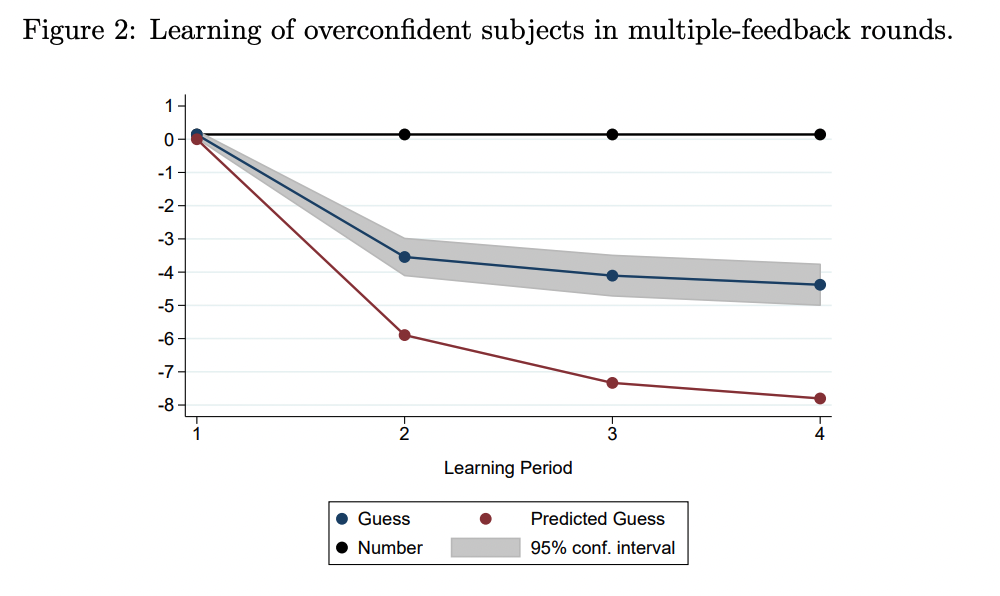
\includegraphics[scale=0.7]{figures/GK_experiment.png}
\end{figure}
    
\end{frame}

\begin{frame}{Results}
    Biased updating in the same direction as the theoretical predictions.\\
    \bigskip
    The bias is not as large as the theory predicts.\\
    \bigskip
    They argue that some agents do update their belief in the ability parameter.\\
    \bigskip
    How are people updating their beliefs on two parameters?
\end{frame}

\begin{frame}{The Research Question}
    We know people fall somewhere between Bayesian Learning and the very extreme Heidhues et al. setting.\\
    \bigskip
    \begin{itemize}
        \item Do the existing alternative theories explain the behavior well?\\
        \begin{itemize}
            \item Is there heterogeneity in how people update their beliefs? (Bayesian, self-attribution, hypothesis testing, self-defeating)
        \end{itemize}
    \bigskip
        \item Can we design an intervention that will help people learn their true type?\\
    \end{itemize}
\end{frame}

\begin{frame}{Theory 2}
    \Large\textbf{ Robust Misspecified Models and Paradigm Shifts \\}
    (Ba, 2022 JMP)
\end{frame}


\begin{frame}{The Setting}
    Same as Theory 1\\
    \bigskip
    Now the entrepreneur entertains an alternative level of ability $\theta'$ (assume $\theta' = \theta^*$).\\
    \bigskip
    Instead of updating $P[\theta]$ every period, they perform a Bayesian hypothesis test:\\
    \bigskip
    Adopt model $\theta'$ at time t iff \\
    $$\frac{\ell_t (\theta')}{\ell_t(\theta)}>\alpha\geq1$$

    Where $$\ell_t(\theta) := \sum_{\omega}g_0(\omega)\prod_{\tau=0}^{t-1}\pi^\theta(y_\tau|a_\tau, \omega)$$
  
\end{frame}

\begin{frame}{Results}

    The self-defeating trap is difficult to escape when the entrepreneur is overconfident.\\
    \bigskip
    Underconfident agents escape the trap at a higher rate than overconfident and learn the true parameter.\\
    \bigskip
    Explains why underconfidence is less prevalent in the data.\\
    \bigskip
    Overconfident agents can escape the trap if their prior is not too "tight" around a self confirming equilibrium.
  
\end{frame}

\begin{frame}{Theory 3: Motivated Beliefs}
    \Large\textbf{Optimal Expectations}\\
    (Brunnermeier and Parker, 2005)\\
    \bigskip
    \Large\textbf{What to blame? Self-serving attribution bias with
multi-dimensional uncertainty}\\
    (Coutts et al., 2022 wp)
\end{frame}

\begin{frame}{The Setting}
    Assume $e$ is fixed and $\theta \in \{\underline{\theta}, \Bar{\theta}\}$ \\
    \bigskip
    Let the probability of success be increasing in $\theta$ and $\omega$ and denote it by by
    $$q(\theta, \omega):=Pr[success|\theta, \omega]$$
    After a success the agent updates their belief about $\theta$ with distortion $\gamma_\theta$:
    $$p_{t+1}(\Bar{\theta}|success)= \frac{\gamma_\theta\pi_t(\Bar{\theta})\sum_\omega g_t(\omega) q_t(\Bar\theta, \omega)}{\gamma_\theta\pi_t(\Bar{\theta})\sum_\omega g_t(\omega)q_t(\Bar{\theta}, \omega)+ \pi_t(\underline {\theta})\sum_\omega g_t(\omega) q_t(\underline{\theta}, \omega)}$$
    
\end{frame}

\begin{frame}{Predictions and Evidence (Coutts et al. 2022)}
    Prediction: Even unbiased agents will overweight $\theta
_H$ after a success and end up being biased.\\
    \bigskip
    Experiment: Evidence of biased updating when $\theta$ is ego-relevant.\\
    \bigskip
    The framework does not allow direct comparisons with the other two theoretical predictions.\\
    \bigskip
    It rationalizes the formation of overconfident beliefs.
    
    
\end{frame}

\begin{frame}{A framework where we can compare}
    Theories 1 and 2 draw conclusions within the same setting already.\\
    \bigskip
    Can we bring the self-serving attribution bias into that setting?\\
    \begin{enumerate}
        \item A larger $\alpha$ in Theory 2 is consistent with self-serving beliefs when the update is done by evaluating the likelihood ratio.
        \item We can write out the fully Bayesian update within the setting and introduce the bias as in Theory 3.
        \item If some subject starts out with the correct belief $\theta$ and ends up being overconfident, it is evidence of a self-serving bias.
    \end{enumerate}
\end{frame}

\begin{frame}{A Theory-Inspired intervention}
    The parameters in this setting are identified. Allowing for a trade-off between exploitation and experimentation is sufficient for learning. \\
    \bigskip
    There are two ways in which experimentation can lead to correct learning:\\
    \begin{enumerate}
        \item Experimentation on $e$:
        \begin{itemize}
            \item Götte and Kozakiewicz show that some agents do learn (are they experimenting?)
            \item Would overconfident/underconfident subjects choose to experiment if the option is made explicitly available to them?
        \end{itemize}
        \bigskip
        \item Allowing experimentation over $\omega$ (switching environments): 
        \begin{itemize}
            \item Hesterman and Le Yaouanq (2021) show that in a model with fixed $e$ and the possibility to experiment in different environments, overconfident subjects learn $\theta$ faster than unbiased/underconfident subjects
        \end{itemize}
    \end{enumerate}
\end{frame}

\begin{frame}{Testing in the lab}

Part 1: Test\\
\begin{itemize}
    \item Get the ego-relevant parameter
    \item Elicit beliefs
\end{itemize}
\pause
Part 2: Investment game (N rounds)\\
\begin{itemize}
    \item Treatment is paid according to their own score as $\theta$ 
    \item Control is paid according to an ego-neutral parameter 
\end{itemize}
\begin{enumerate}
    \item Choose an amount e to invest
    \item Returns are $\theta \omega + e(\omega-\frac{1}{2}e) + \varepsilon_t$
    \item Belief elicitation
\end{enumerate}
\pause
Part 3: Explicitly allow experimentation
\begin{itemize}
    \item Draw a random $e$ for the next $n$ rounds
    \item Draw a new return parameter $\omega$
\end{itemize}

\end{frame}

\begin{frame}{What needs to be done}
    \begin{enumerate}
        \item Define self-serving attribution bias in the framework of theories 1 and 2 (??)\\
        \bigskip
        \item Get predictions in a simplified environment (finite parameter sets).
        \bigskip
        \item Parameters should be such that there are differences among models:
        \begin{itemize}
            \item Subjects update in Theory 2 but fall into self-defeating eq. in Theory 1
            \item Self-serving beliefs make the default model more sticky in Theory 2 
            \item Self serving bias over weights high $\theta$ relative to the Bayesian
            \item Under self serving bias, unbiased subjects become biased. And overconfident subjects become more confident after a success
        \end{itemize}
    \end{enumerate}
\end{frame}

\begin{frame}{The end}
    \large\textbf{Thank you!}
\end{frame}

\end{document}
